\documentclass[ignoreonframetext,unicode]{beamer}

\usepackage[utf8]{inputenc}
\usepackage[T1]{fontenc}
\usepackage[english,russian]{babel}
\usepackage{cmap}
\usepackage{amsmath}
\usepackage{amsfonts}
\usepackage{amssymb}
\usepackage{graphicx,pgf}
\usepackage{multimedia}


\usepackage{color,soul}
\usepackage{multirow}
\usepackage{supertabular}
\usepackage{multicol}
\usepackage{subcaption}
\usepackage{float}
\usepackage{xcolor,colortbl}
\graphicspath{{./style/}{./figures/}}
%\usetheme{Copenhagen}
%\usetheme{default}
%\usetheme{Boadilla}
%\usetheme{Madrid}
%\usetheme{AnnArbor}
\usetheme{Warsaw}
%\usetheme{CambridgeUS}
%\usetheme{Pittsburgh}

\useinnertheme{circles}   %внутренняя тема
%\useoutertheme{smoothbars}   %внешняя тема
\usecolortheme{seahorse}     %цветовая схема
%\usefonttheme{serif}    %шрифты
%\defbeamertemplate*{footline}{shadow theme}
%\setbeameroption{hide notes}

%номера слайдов
\newcommand*\oldmacro{}%
\let\oldmacro\insertshorttitle%
\renewcommand*\insertshorttitle{%
	\oldmacro\hfill%
	\insertframenumber\,/\,\inserttotalframenumber}
\RequirePackage{caption}
\DeclareCaptionLabelSeparator{defffis}{ }
\captionsetup{justification=centering,labelsep=defffis}

\institute[каф. Прикладная математика ФН-2]{группа ФН2-42Б}
\date{\today}
\titlegraphic{
\includegraphics[width=2cm]{emblema.pdf}}
%\renewcommand{\vec}[1]{\text{\mathversion{bold}${#1}$}}

%\title[Задача об ограниченном ранце]{Задача об ограниченном ранце. Метод ветвей и~границ и динамическое программирование}
\title[Задача об ограниченном ранце]{Задача об ограниченном ранце.}
%\author[Абрамов З.\,И., Швецов Г.\,A.]{Абрамов З.\,И.\and\\[0.5mm] Швецов Г.\,А.}
\author[Абрамов З.И., Швецов Г.A.]{Абрамов З.И.\and\\[0.5mm] Швецов Г.А.}

\frenchspacing
\righthyphenmin=2

\usepackage{comment}

\begin{comment}
	Красивый блок с заголовком title (если он пустой, то заголовка не будет)
	\begin{block}{title}
		содержимое...
	\end{block}
\end{comment}

\begin{comment}
	Колонки
	https://latex-beamer.com/tutorials/columns/
	
	\begin{columns}
		\begin{column}{0.5\textwidth}
			содержимое...
		\end{column}
		
		\begin{column}{0.5\textwidth}
			содержимое...
		\end{column}
	\end{columns}
	
	Отступ можно сделать добавив третью колонку между ними (тут же можно сделать разделитель):
	\begin{column}{0.01\textwidth}
		%\rule{.1mm}{0.7\textheight}
	\end{column}
	
\end{comment}

\begin{comment}
	Другие команды:
	\begin{center}
		содержимое...
	\end{center}
	\includegraphics[width=0.5\textwidth]{image_name.png}
	
	Какие-то команды:
	\frametitle{explanation}
\end{comment}

% Выравнивание по ширине
\usepackage{ragged2e}
\justifying

\parindent=0.5cm

%%%%%%%%%%%%%%%%%%%%%%%%%%%%%%%%%%%%%%%%%%%%%%%%%%%%%%%%%%%%
%%%%%%%%%%%%%%%%%%%%%%%%%%%%%%%%%%%%%%%%%%%%%%%%%%%%%%%%%%%%
%%%%%%%%%%%%%%%%%%%%%%%%%%%%%%%%%%%%%%%%%%%%%%%%%%%%%%%%%%%%

\begin{document}
	\begin{frame}[plain]
		\maketitle	\end{frame}
		\section{Постановка задачи}
	\begin{frame}{Постановка задачи}	
		\small
		Пусть имеется $n$ типов предметов. Каждый тип предмета $i$ характеризуется весом $w_i$ и стоимостью $c_i$ одного предмета и количеством предметов $k_i$ данного типа. Также имеется рюкзак вместимости $W$.
		
		Требуется собрать набор с максимальной полезностью таким образом, чтобы он имел вместимость не больше $W$. При этом количество предметов типа $i$ не должно превышать $k_i$.
		
		В математической форме:
		\begin{gather*}
			\sum_{i=1}^{n} c_i x_i \to \max \\
			\sum_{i=1}^{n} w_i x_i \leqslant W \\
			\forall i\in\{1,\dots,n\} \quad x_i \in \{0,\dots, k_i\}
		\end{gather*}
	\end{frame}
		\section{Метод ветвей и границ}
	\begin{frame}{Метод ветвей и границ}
		\begin{columns}
			\column{0.5\textwidth}
			\begin{figure}[H]
			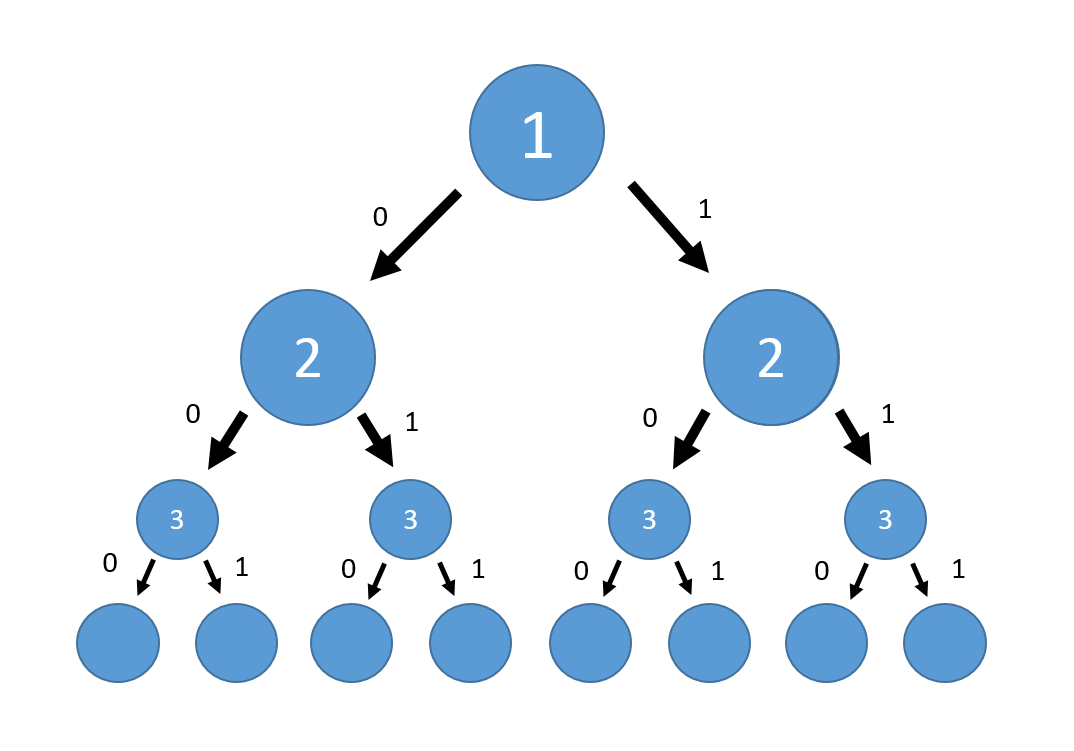
\includegraphics[scale=0.2]{Дерево}
			\small
		Дерево полного перебора, соответствующее поиску решения для трех предметов.
		\end{figure}
			\column{0.5\textwidth}
	Метод ветвей и границ является вариацией метода полного перебора с той разницей, что исключаются заведомо неоптимальные ветви дерева полного перебора.
		\end{columns}
				\end{frame}
			
			
		\begin{frame}{Метод ветвей и границ}
			\begin{figure}[H]
				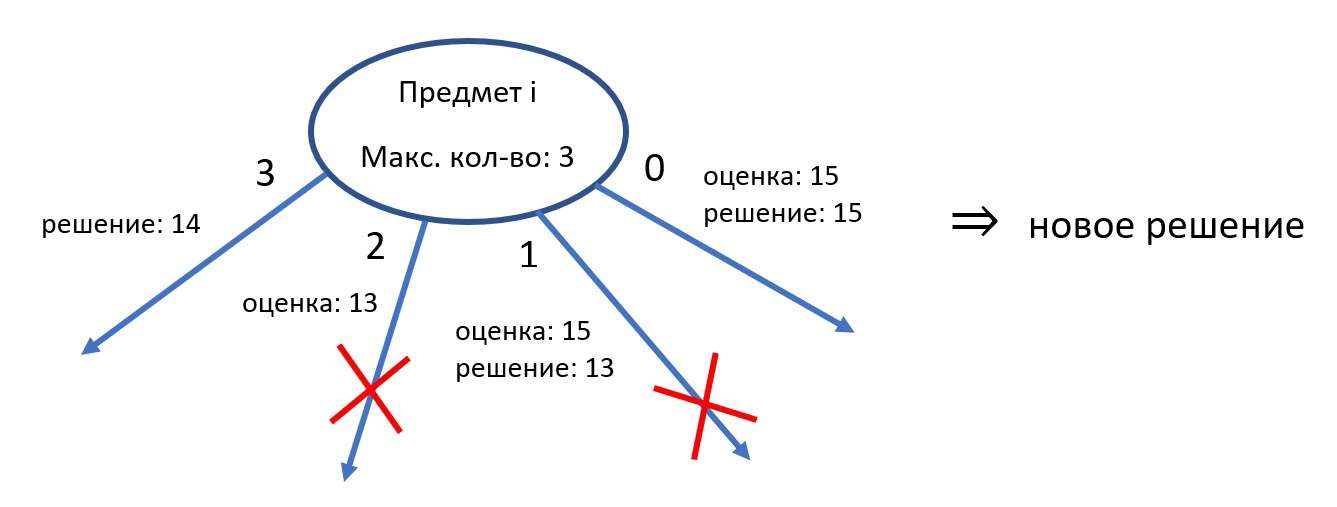
\includegraphics[scale=0.23]{мвг}
			\end{figure}
			\end{frame}
		
		
	% TODO другие слайды
	\section{Динамическое программирование}
	\begin{frame}{Динамическое программирование}
	Подход динамического программирования состоит в том, что если при решении исходной задачи часто решаются одинаковые подзадачи, то имеет смысл сохранять решение таких подзадач, сократив тем самым количество вычислений. 
	\begin{figure}[H]
		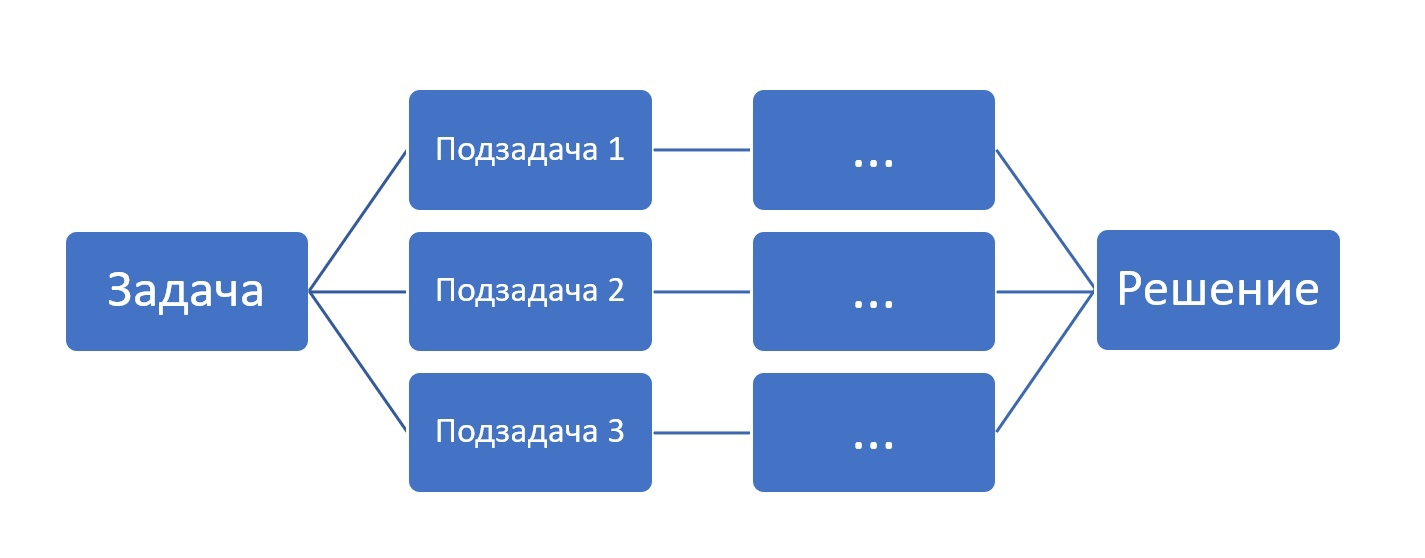
\includegraphics[scale=0.23]{дп}
	\end{figure}
	\end{frame}
			
	\begin{frame}{Динамическое программирование}
		В качестве таких подзадач будем решать задачу о ранце для первых $n’<n$ предметов и рюкзака вместимости $W’<W$.
			\begin{columns}
			\column{0.4\textwidth}
			\begin{figure}[H]
				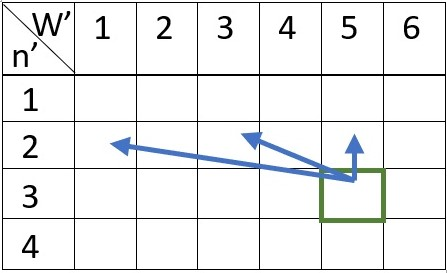
\includegraphics[scale=0.37]{таблица}
			\end{figure}
			\column{0.6\textwidth}
			\begin{gather*}
				W=6,\quad n=4; \\
				n'=3,\quad W'=5;\\
				w_3=2,\quad k_3=2;\\
				dp[3,4]=\max_{x_i=0,1,2}(x_i\cdot c_3+dp[2,4-x_i\cdot2]).
				\end{gather*}
		\end{columns}
	\end{frame}
	
	% TODO другие слайды
	\section{Пример работы}	
	\begin{frame}{Пример работы}
	Пример с двумя решениями при $\textrm{max\_weight}=1000$.	\begin{figure}[H]
			\centering
			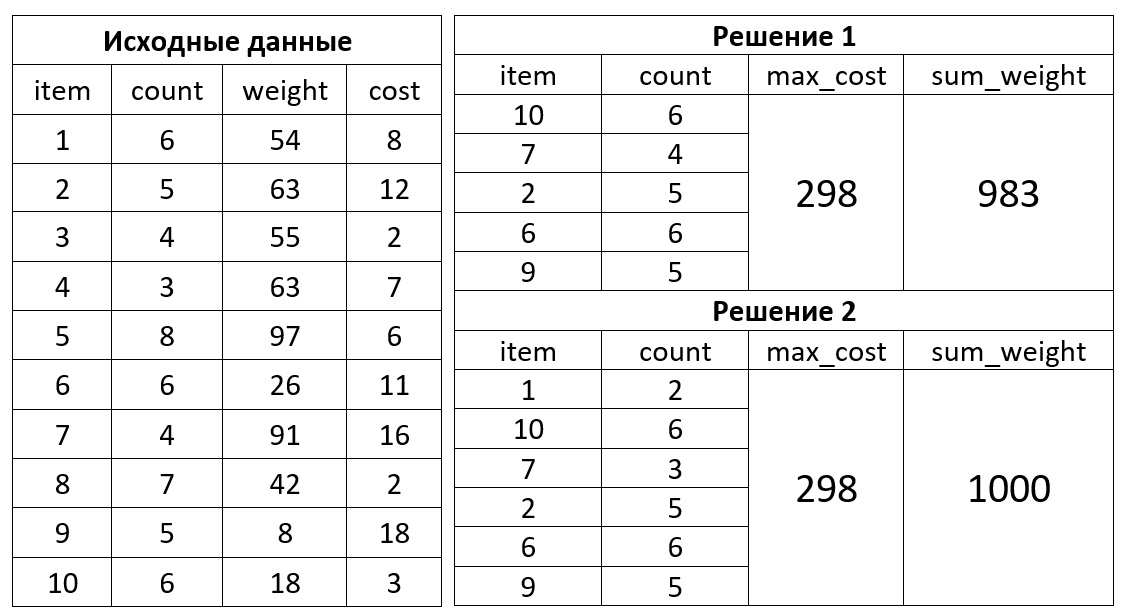
\includegraphics[scale=0.25]{пример}
		\end{figure}	
	\end{frame}

	
	% TODO время исполнения зависит еще от максимального веса
	\section{Время исполнения методов}
	\begin{frame}{Время исполнения методов на C++}
			\begin{figure}[H]
			\centering
			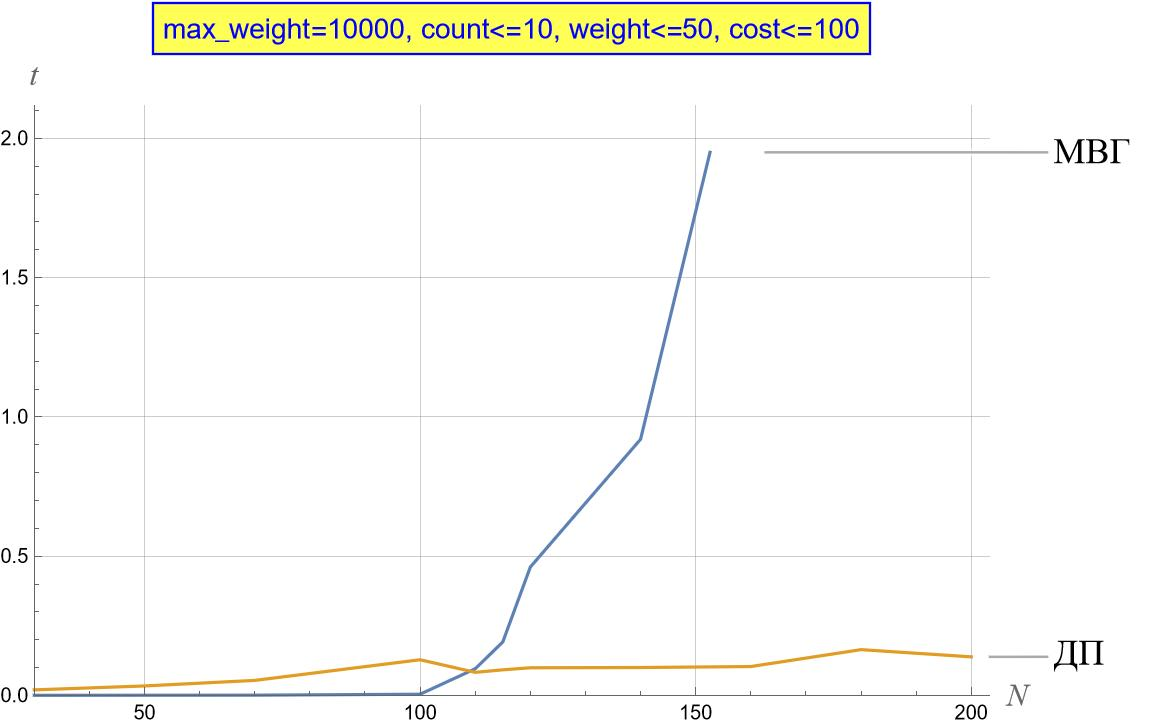
\includegraphics[scale=0.5]{plot4}
		\end{figure}	
	\end{frame}
	
	\begin{frame}{Время исполнения методов на Wolfram Mathematica}
		\begin{figure}[H]
			\centering
			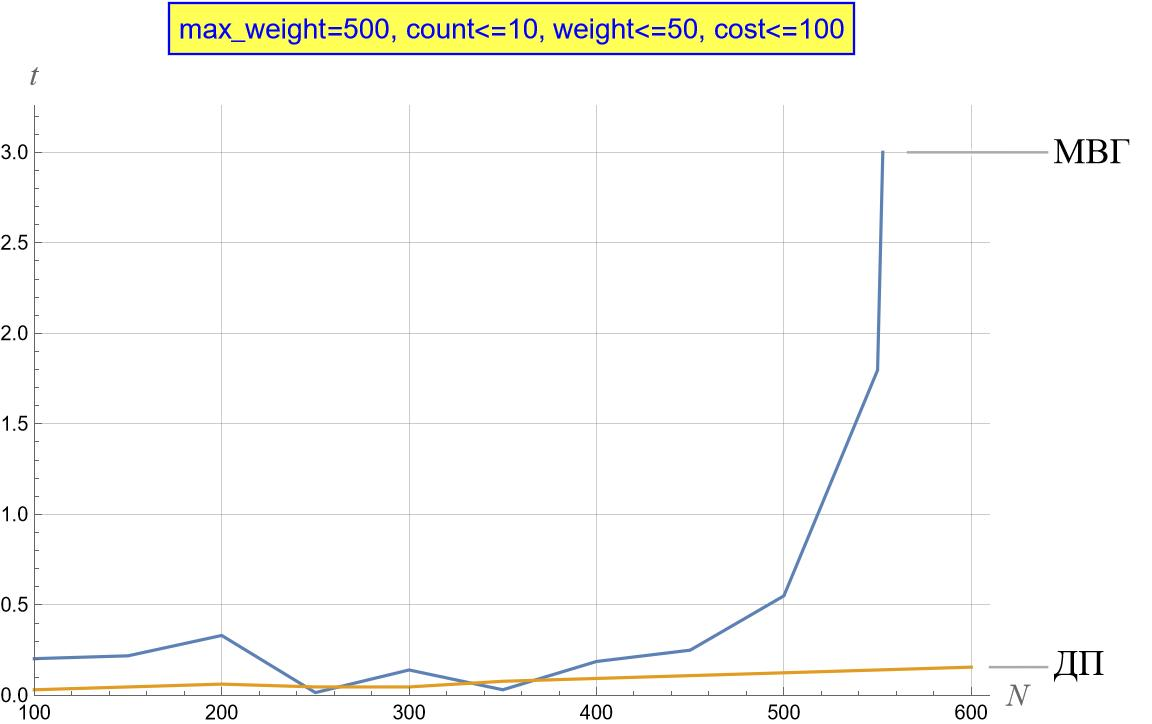
\includegraphics[scale=0.5]{plot5}
		\end{figure}	
	\end{frame}
	
	\begin{frame}
		\LARGE
		\centering
		Спасибо за внимание!
	\end{frame}
	
\end{document}